\section{Multi-Layer Perceptron}
Per l'addestramento è stato utilizzato il package R \texttt{mxnet}.

\subsection{Holdout}
Le misure di accuracy, precision, recall e F-measure sono le seguenti:
\begin{figure}[H]
	\centering
	\begin{tabular}{llcccc}
		\toprule
		&& \textbf{Accuracy} & \textbf{Precision} & \textbf{Recall} & 
		\textbf{F-Measure}  \\
		\midrule
		\multirow{1}{*}{ReLU} 
			& Training 		& 93,91\% & 82,62\% & 33,31\% & 47,48\%		\\ 
			& Validation	& 92,51\% & 64,82\% & 29,25\% & 40,31\%		\\
		\midrule
		\multirow{1}{*}{Sigmoide} 
			& Training 		& 92,08\% & 71,70\% & 67,70\% & 12,37\%		\\ 
			& Validation	& 91,80\% & 81,08\% & 68,03\% & 12,55\%		\\
		\bottomrule
	\end{tabular}
	\captionof{table}{Analisi performance con holdout}
	\label{tab:mlp_h_r_performance}
\end{figure}

Di seguito vengono mostrate le curve ROC rispettivamente sul training set e sul 
validation set:

\begin{figure}[H]
	\centering
	\begin{subfigure}[t]{1\textwidth}
		\begin{minipage}[t]{0.475\textwidth}
			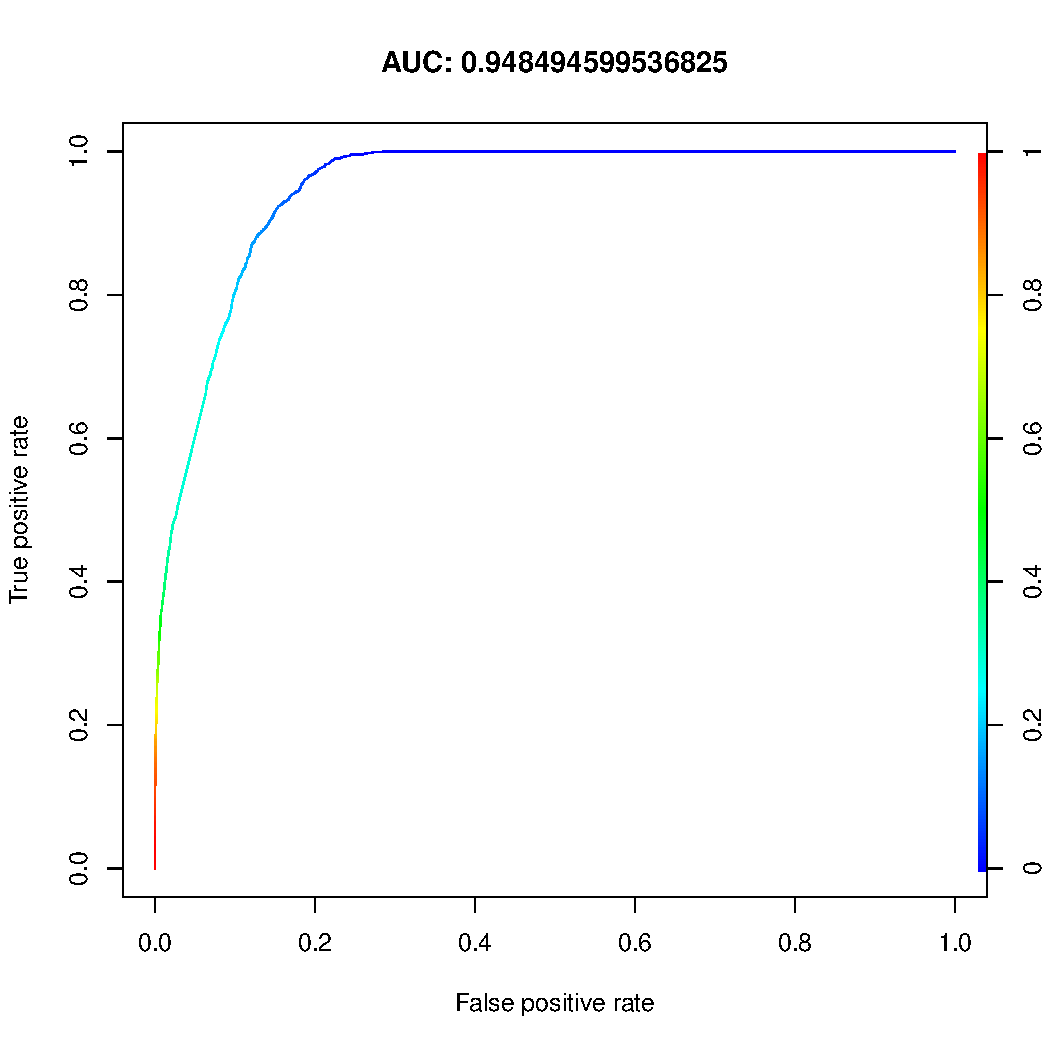
\includegraphics[width=\textwidth]{images/ml/mlp/holdout/relu-training}
		\end{minipage}
		\hfill
		\begin{minipage}[t]{0.475\textwidth}
			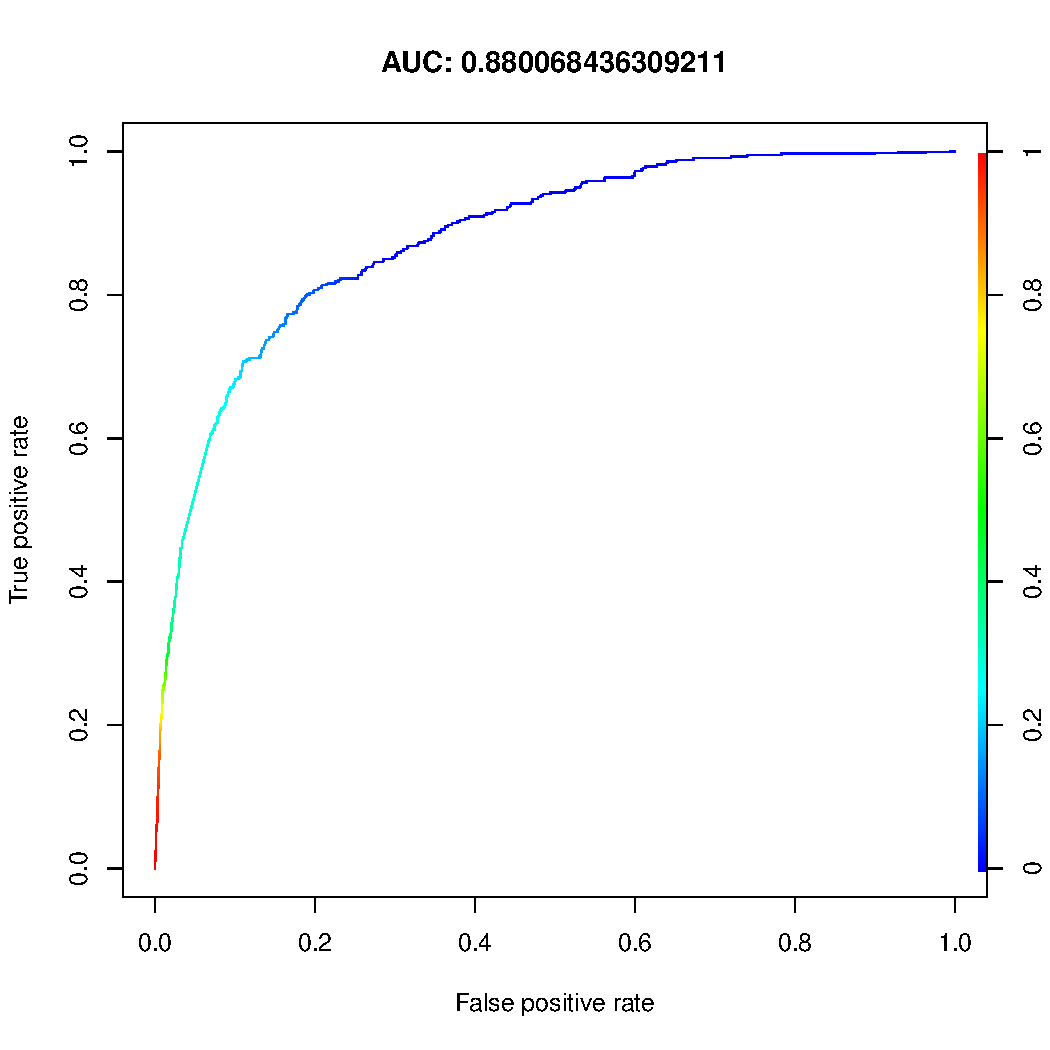
\includegraphics[width=\textwidth]{images/ml/mlp/holdout/relu-test}
		\end{minipage}
	\end{subfigure}
	\caption{Curve ROC del modello ReLU su training e validation set}
	\label{fig:mlp_h_r_roc}
\end{figure}

\begin{figure}[H]
	\centering
	\begin{subfigure}[t]{1\textwidth}
		\begin{minipage}[t]{0.475\textwidth}
			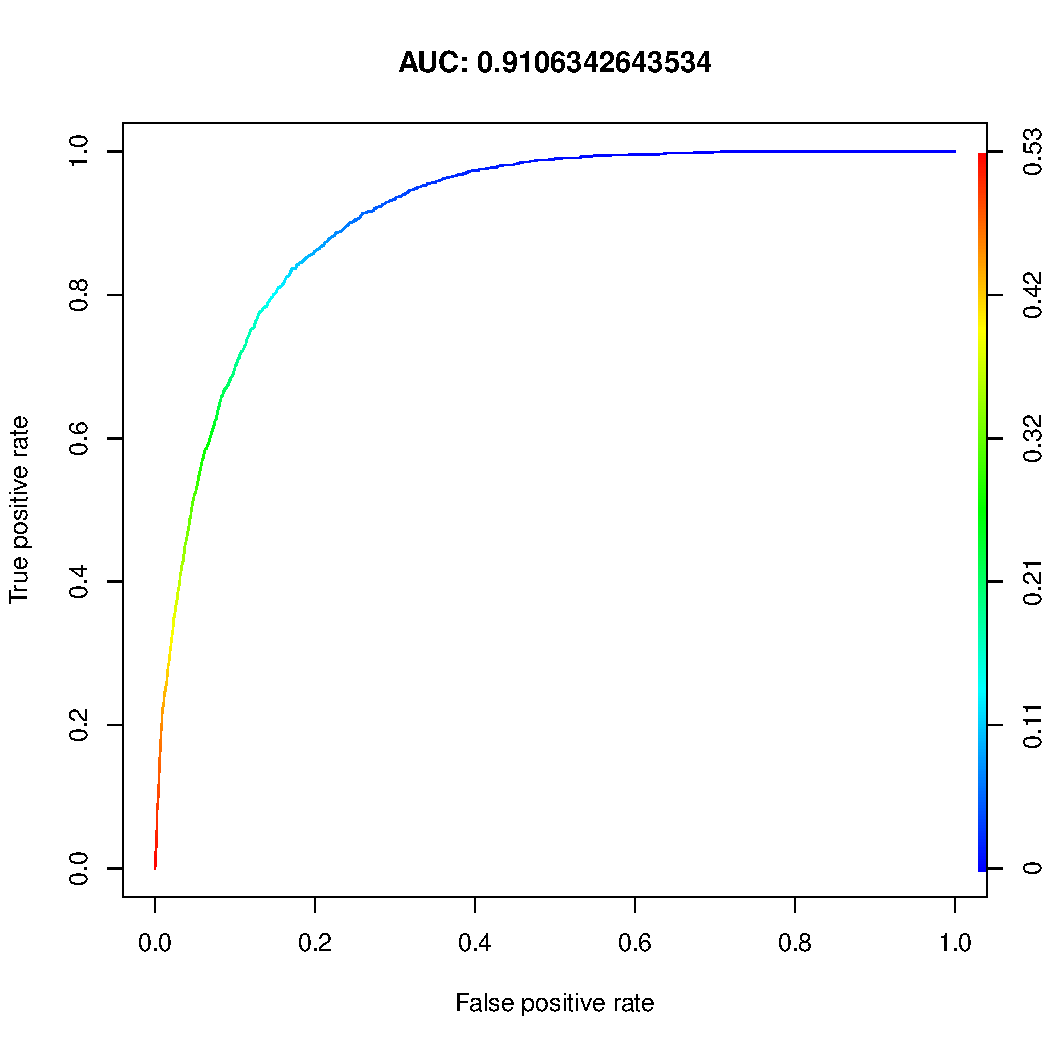
\includegraphics[width=\textwidth]{images/ml/mlp/holdout/sigmoid-training}
		\end{minipage}
		\hfill
		\begin{minipage}[t]{0.475\textwidth}
			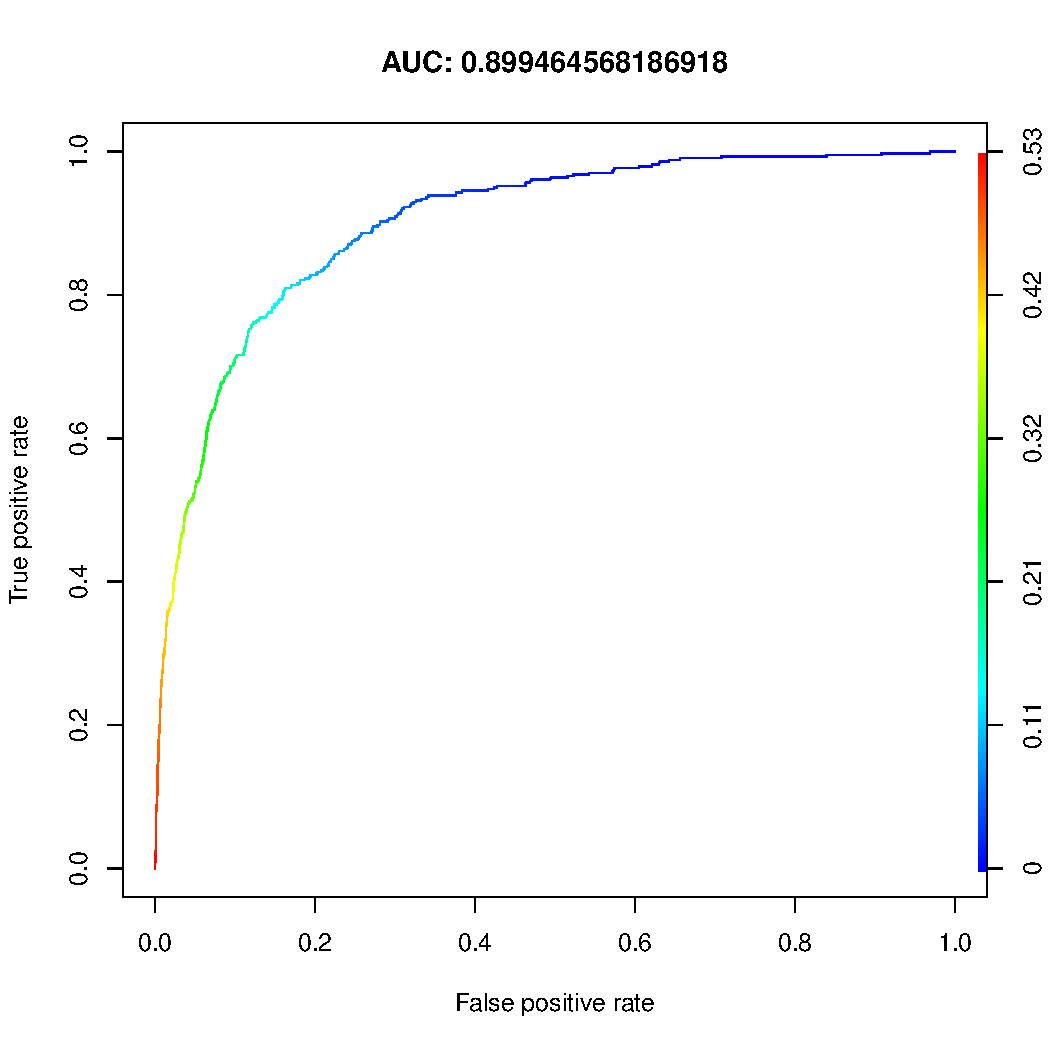
\includegraphics[width=\textwidth]{images/ml/mlp/holdout/sigmoid-test}
		\end{minipage}
	\end{subfigure}
	\caption{Curve ROC del modello sigmoide su training e validation set}
	\label{fig:mlp_h_s_roc}
\end{figure}

\subsection{10-fold Cross Validation}

Vengono mostrate nella Tabella~\ref{tab:mlp_cv_fold_performance} i dati 
relativi ai singoli fold e in tabella \ref{tab:mlp_cv_performance} le misure 
complessive di accuracy, precision, recall e F-measure, calcolate come media 
delle misure di ogni fold. 

\begin{figure}[H]
	\centering
	\begin{tabular}{llrrrr}
		\toprule
		&& \textbf{Accuracy} & \textbf{Precision} & \textbf{Recall} & 
		\textbf{F-Measure}  \\
		% \midrule
		% \multirow{10}{*}{Training} & Fold1 & 94,23\% & 84,42\% & 40,57\% & 
		% 54,80\% \\
		% & Fold2 & 94,43\%  & 84,30\% & 43,81\% & 57,65\% \\
		% & Fold3 & 94,17\%  & 85,68\% & 37,93\% & 52,59\% \\
		% & Fold4 & 94,09\%  & 85,98\% & 39,02\% & 53,68\% \\
		% & Fold5 & 94,38\%  & 85,22\% & 39,86\% & 54,32\% \\
		% & Fold6 & 93,99\%  & 85,52\% & 37,46\% & 52,10\% \\
		% & Fold7 & 94,53\%  & 85,00\% & 36,83\% & 51,40\% \\
		% & Fold8 & 94,72\%  & 87,09\% & 40,01\% & 54,83\% \\
		% & Fold9 & 94,37\%  & 84,93\% & 35,51\% & 50,08\% \\
		% & Fold10 & 94,50\% & 86,60\% & 35,77\% & 50,63\%  \\
		\midrule
		\multirow{10}{*}{Validation} 
				& Fold 1  & 94,07\% &   0,00\% &  0,00\% &    ND   \\
				& Fold 2  & 94,58\% &  53,33\% &  5,76\% & 10,39\% \\
				& Fold 3  & 93,84\% &  77,27\% & 10,06\% & 17,80\% \\
				& Fold 4  & 95,76\% &  72,73\% & 70,80\% & 12,90\% \\
				& Fold 5  & 92,27\% &  62,50\% &  4,98\% &  9,22\% \\
				& Fold 6  & 95,29\% &  71,43\% &  4,07\% &  7,69\% \\
				& Fold 7  & 87,52\% &  59,46\% &  6,77\% & 12,15\% \\
				& Fold 8  & 90,03\% &  68,48\% & 21,88\% & 33,16\% \\
				& Fold 9  & 89,40\% &  74,19\% & 15,33\% & 25,41\% \\
				& Fold 10 & 87,56\% & 100,00\% &  0,63\% &  1,25\% \\
		\bottomrule 
	\end{tabular}
	\captionof{table}{Analisi delle performance per singolo fold}
	\label{tab:mlp_cv_fold_performance}
\end{figure}

\begin{figure}[H]
	\centering
	\begin{tabular}{lcccc}
		\toprule
		& \textbf{Accuracy} & \textbf{Precision} & \textbf{Recall} & 
		\textbf{F-Measure}  \\
		\midrule
		% Training	&  94,34\% & 85,47\% & 38,68\%	& 53,21\%  	\\ 
		Validation	&  92,03\%	& 63,94\%	& 14,03\% &	14,44\% \\
		\bottomrule
	\end{tabular}
	\captionof{table}{Analisi performance complessive con cross validation}
	\label{tab:mlp_cv_performance}
\end{figure}

Vengono infine mostrate le curve ROC per ciascun fold, sia sul training che 
sul validation set. Possiamo notare come in nessun fold il modello abbia un 
valore di Area Under Curve (AUC) inferiore al valore 0,80, che viene 
considerato come un indice di buone prestazioni. Si ha un valore medio di 
0,869 con deviazione standard di 0,025.

\begin{figure}[p]
	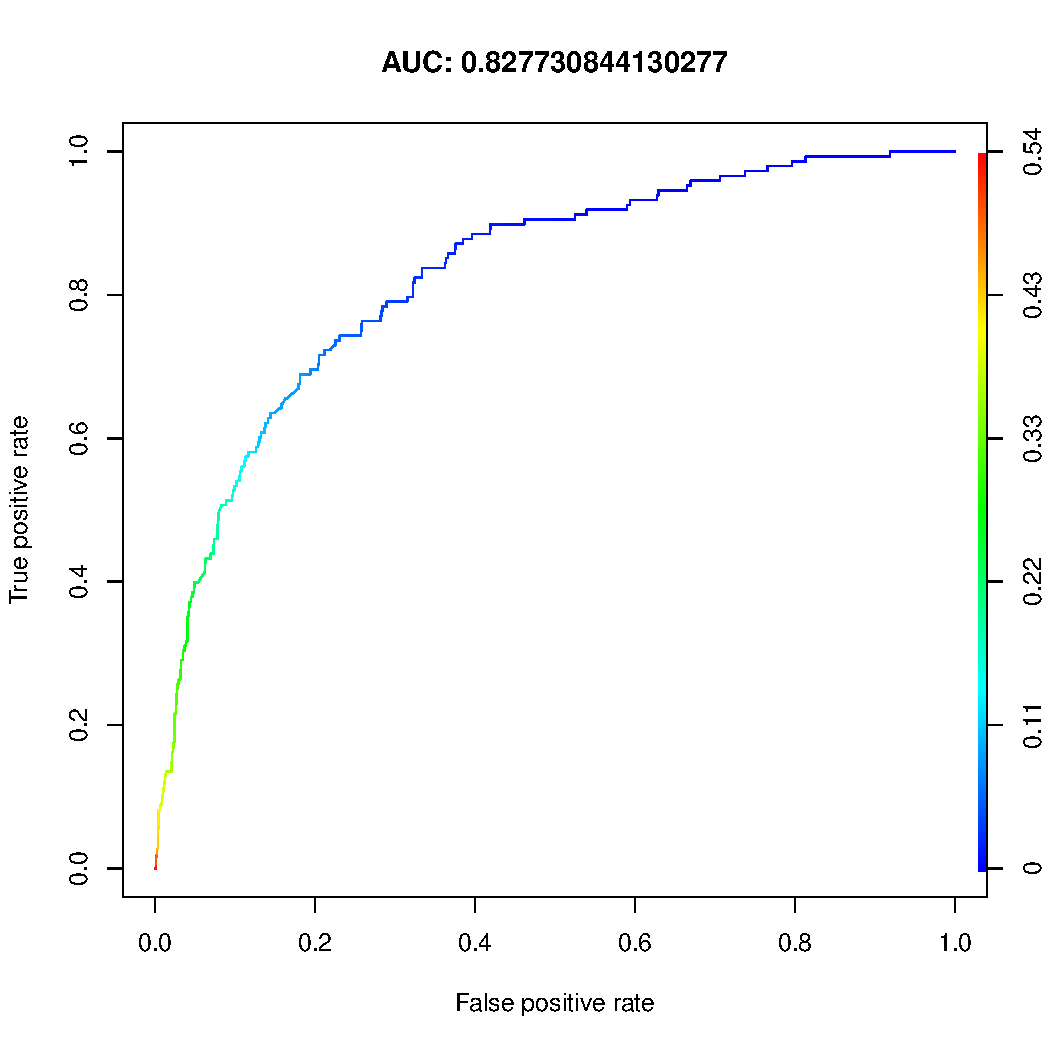
\includegraphics[width=.32\textwidth]{images/ml/mlp/crossval/roc-1.pdf}
	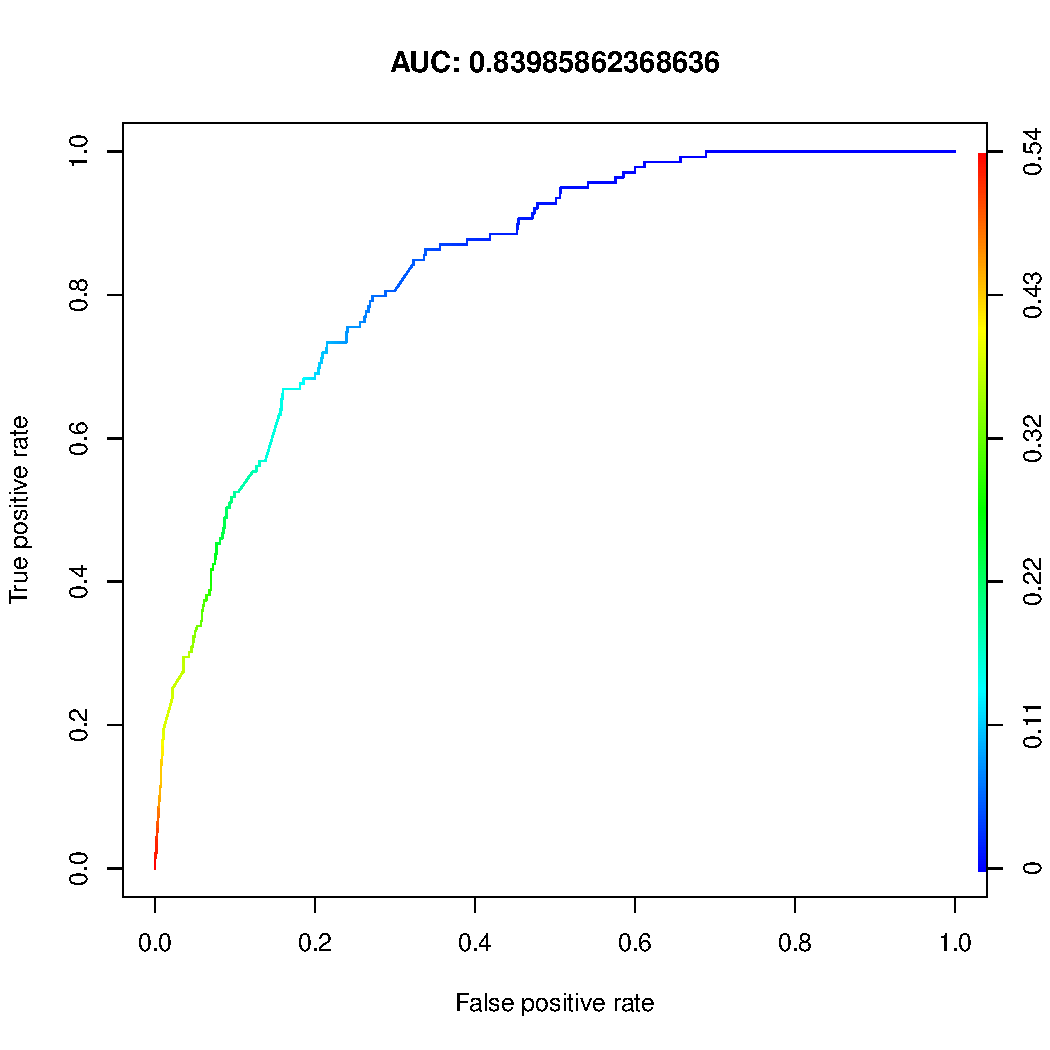
\includegraphics[width=.32\textwidth]{images/ml/mlp/crossval/roc-2.pdf}
	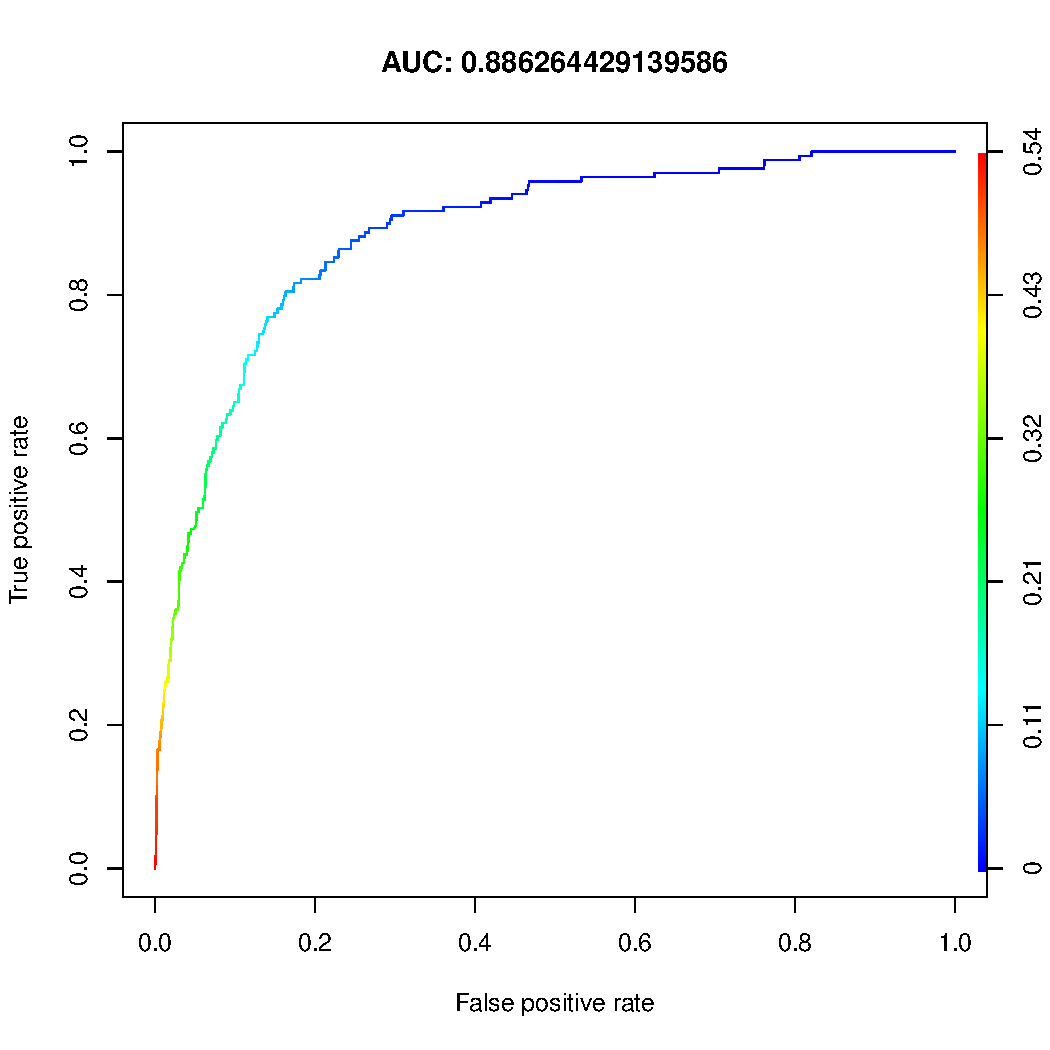
\includegraphics[width=.32\textwidth]{images/ml/mlp/crossval/roc-3.pdf}
	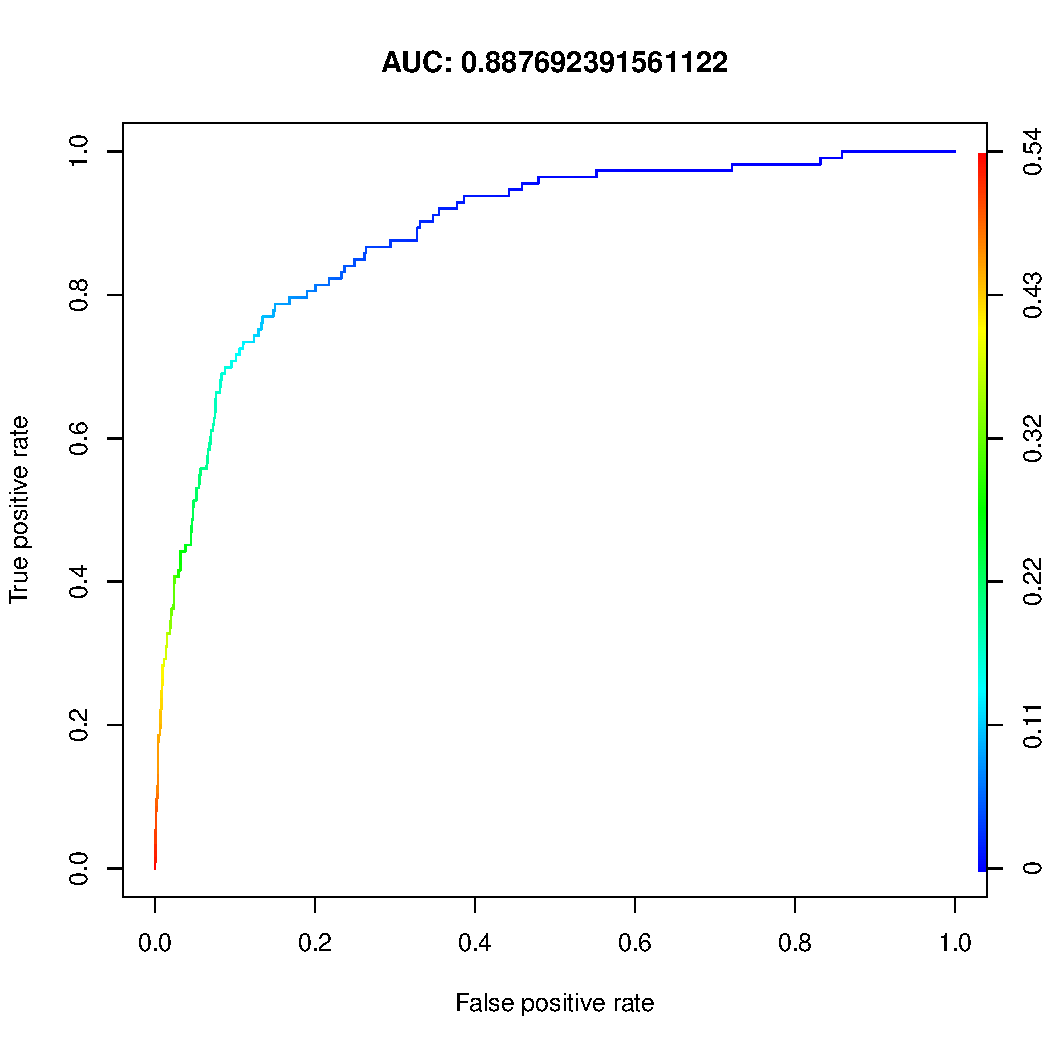
\includegraphics[width=.32\textwidth]{images/ml/mlp/crossval/roc-4.pdf}
	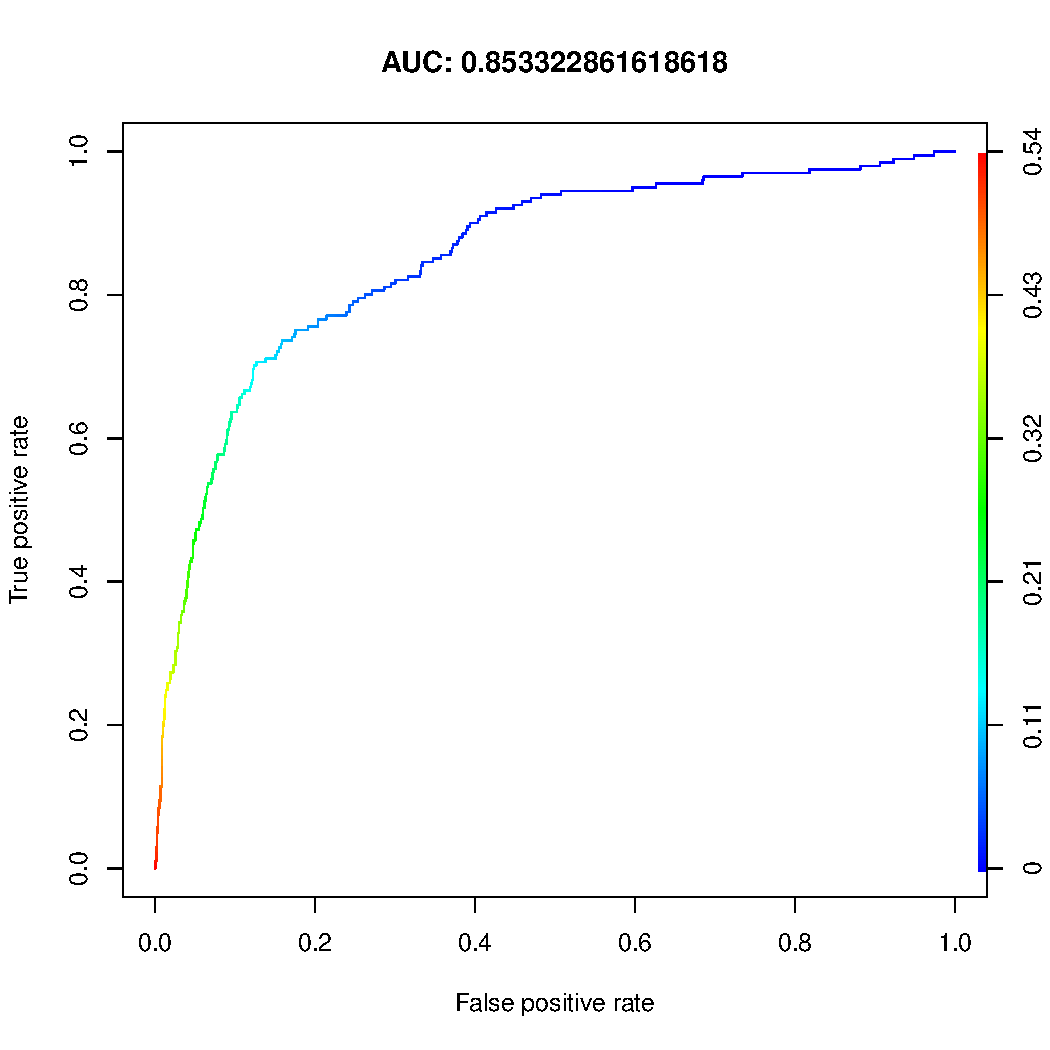
\includegraphics[width=.32\textwidth]{images/ml/mlp/crossval/roc-5.pdf}
	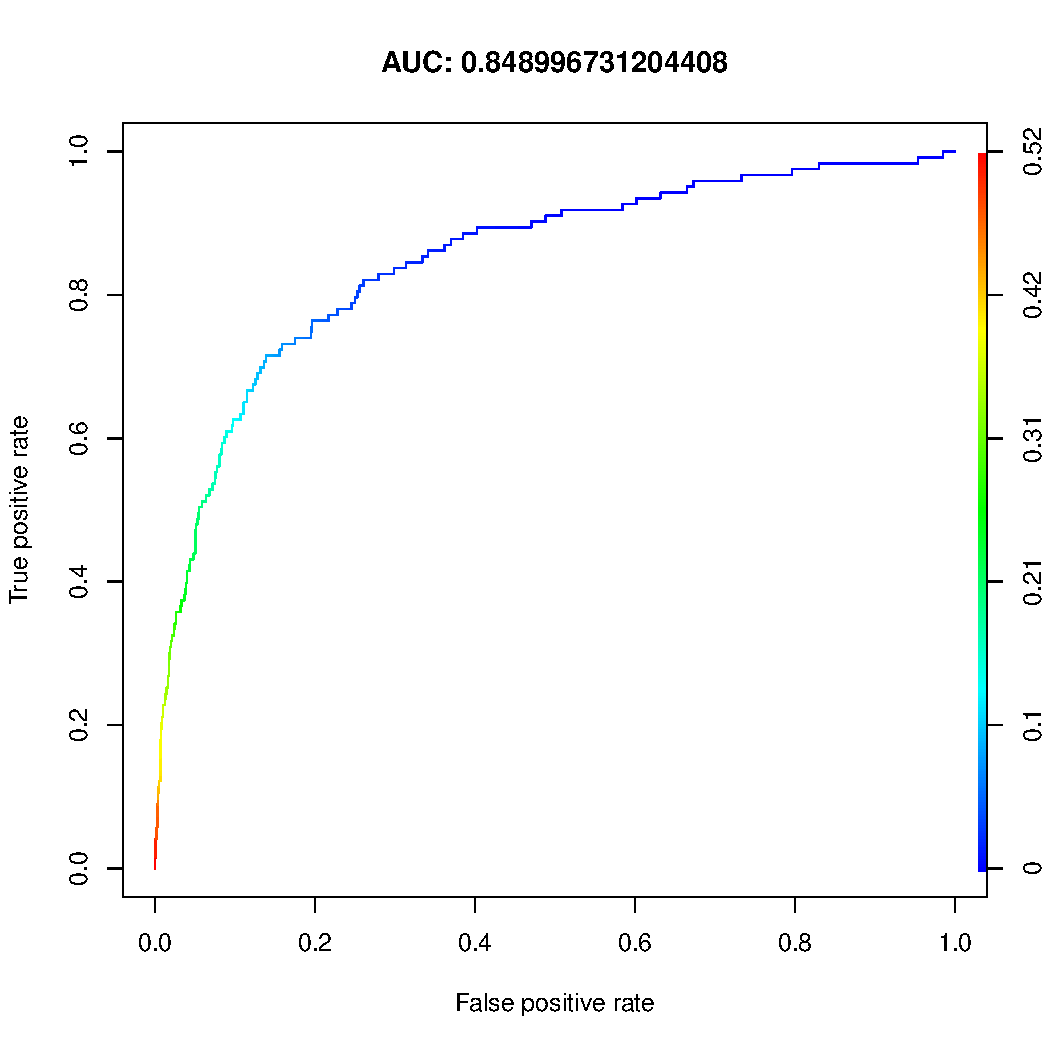
\includegraphics[width=.32\textwidth]{images/ml/mlp/crossval/roc-6.pdf}
	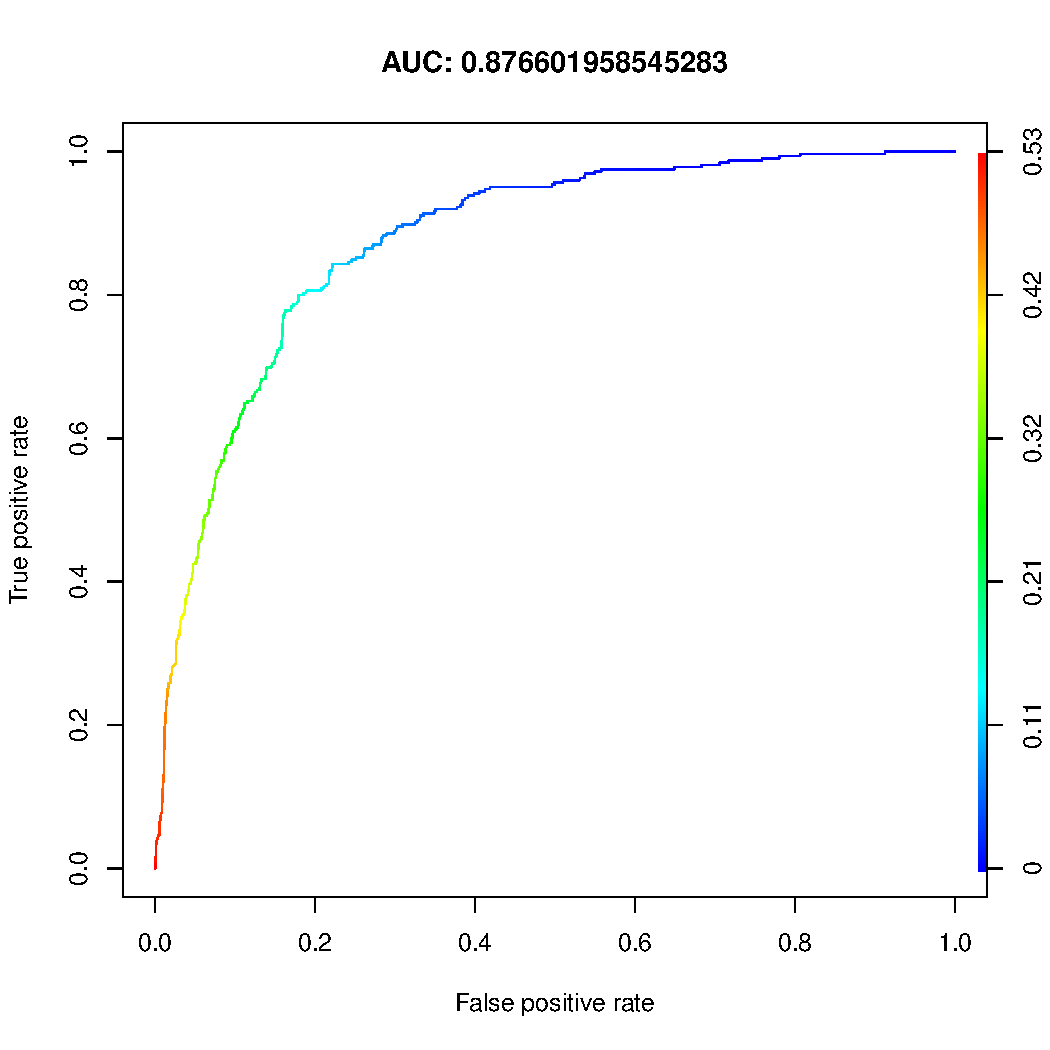
\includegraphics[width=.32\textwidth]{images/ml/mlp/crossval/roc-7.pdf}
	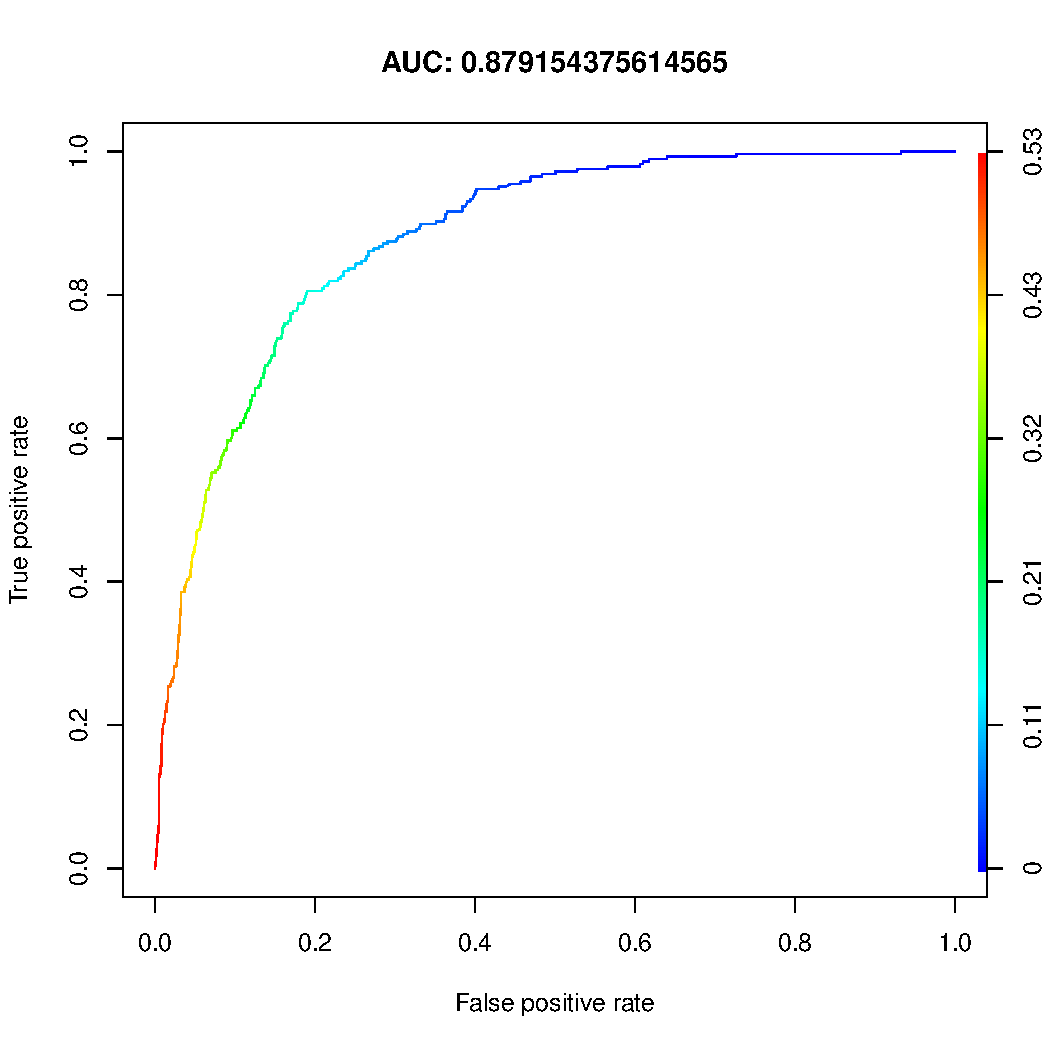
\includegraphics[width=.32\textwidth]{images/ml/mlp/crossval/roc-8.pdf}
	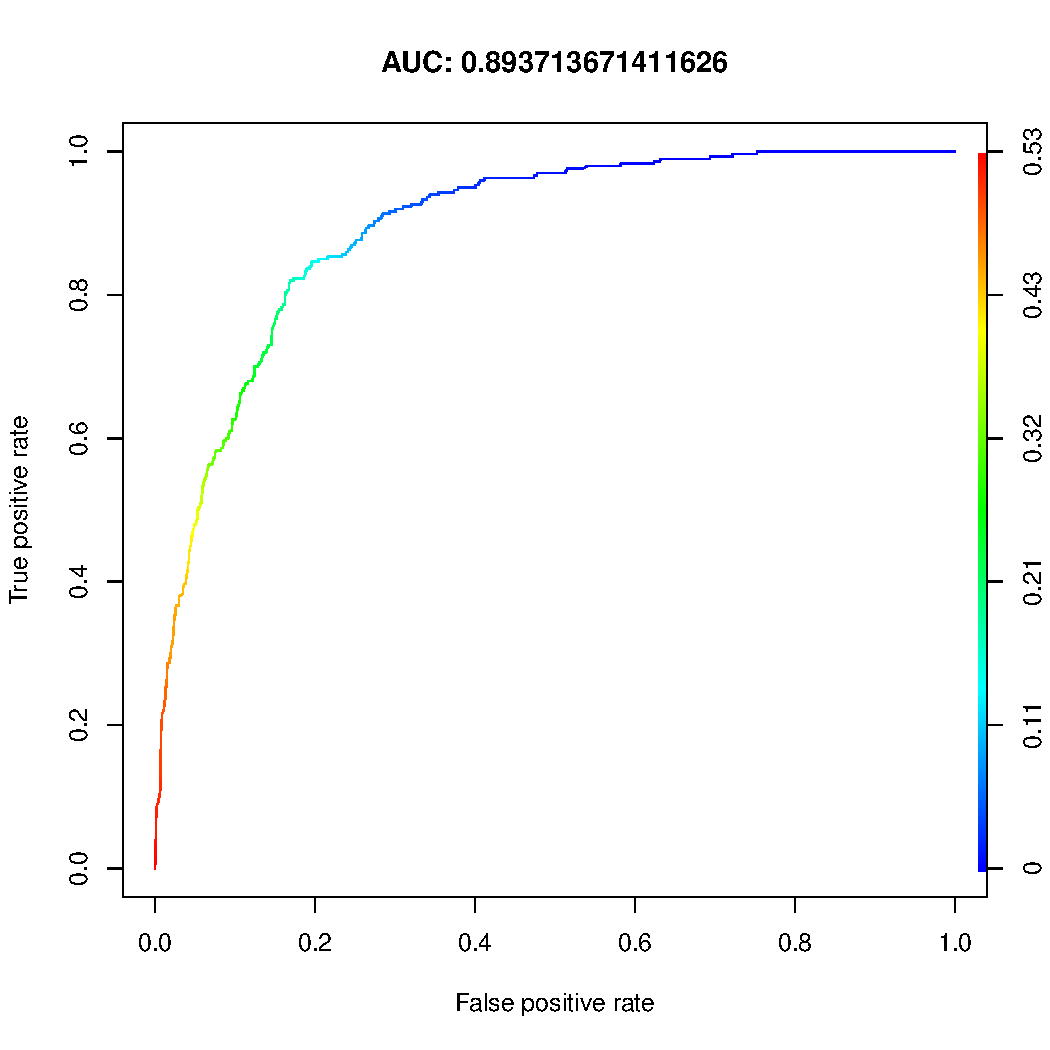
\includegraphics[width=.32\textwidth]{images/ml/mlp/crossval/roc-9.pdf}
	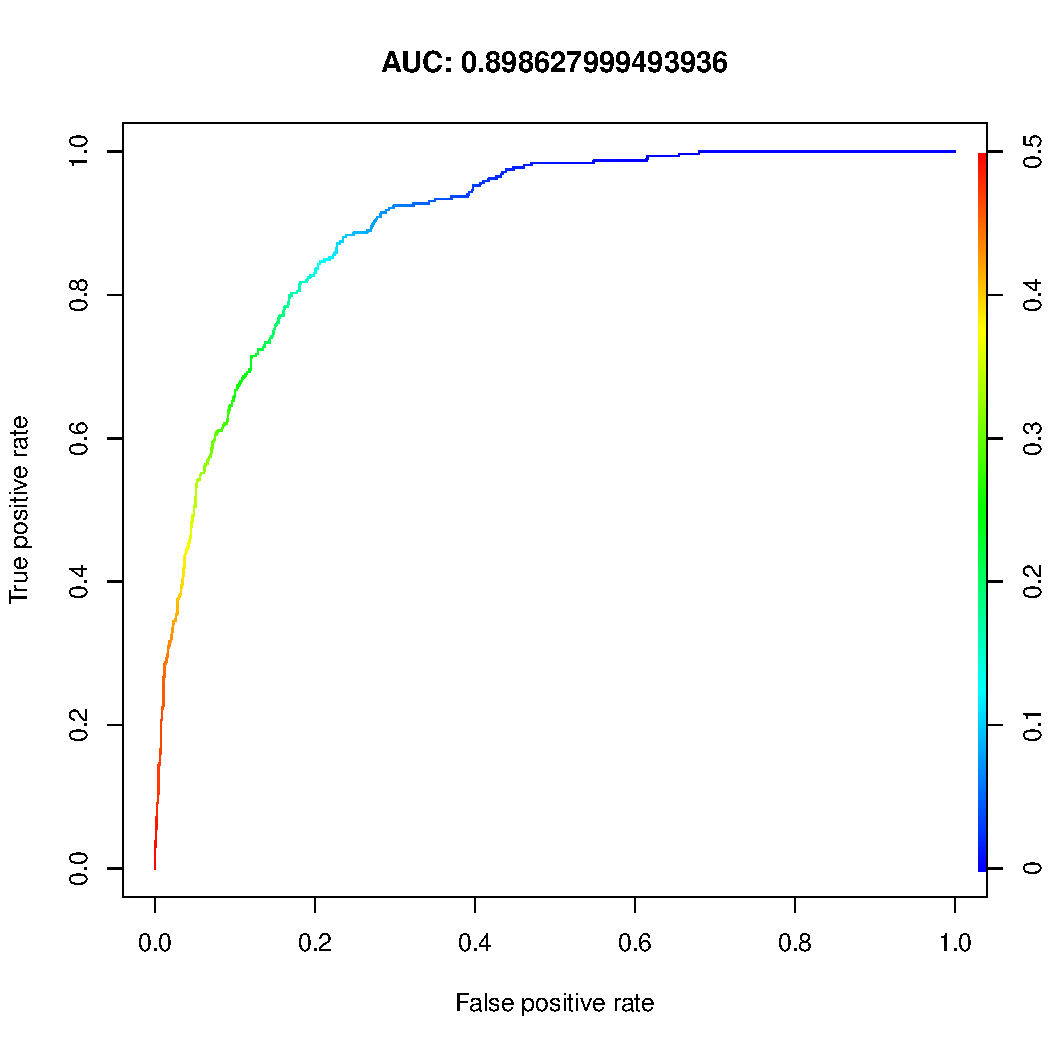
\includegraphics[width=.32\textwidth]{images/ml/mlp/crossval/roc-10.pdf}
	\caption{Curve ROC sul validation set}
	\label{fig:mlp_cv_roc_valid}
\end{figure}
